\documentclass[12pt,a4paper,oneside]{report}

% =========================================================
% COMPILATION NOTE
% =========================================================
% Compile with XeLaTeX or LuaLaTeX because the report uses fontspec
% and Vietnamese Unicode text.

% =========================================================
% PACKAGES
% =========================================================
\usepackage{fontspec}
\IfFontExistsTF{Tinos}{\setmainfont{Tinos}}{\setmainfont{Times New Roman}}
\IfFontExistsTF{Arimo}{\setsansfont{Arimo}}{\setsansfont{Arial}}
\IfFontExistsTF{Noto Sans Mono}{\setmonofont{Noto Sans Mono}}{\setmonofont{Courier New}}

\usepackage[a4paper,left=3.0cm,right=2.2cm,top=2.5cm,bottom=2.5cm]{geometry}
\usepackage{amsmath,amssymb,mathtools}
\usepackage{graphicx}
\usepackage{booktabs,longtable,array,multirow,tabularx}
\usepackage{float}
\usepackage{caption,subcaption}
\usepackage{enumitem}
\usepackage{xcolor}
\usepackage[round,authoryear]{natbib}
\usepackage{hyperref}
\usepackage{fancyhdr}
\usepackage[most]{tcolorbox}
\usepackage{titlesec}
\usepackage{tikz}
\usetikzlibrary{arrows.meta,positioning,shapes.geometric,calc,fit,backgrounds,decorations.pathreplacing}
\usepackage{algorithm}
\usepackage{algpseudocode}
\usepackage{microtype}
\usepackage{setspace}
\usepackage{tocloft}
\usepackage{etoolbox}

\graphicspath{{figures/}}

% =========================================================
% COLORS AND STYLE
% =========================================================
\definecolor{mainblue}{HTML}{1F4E79}
\definecolor{lightblue}{HTML}{EAF2F8}
\definecolor{mainteal}{HTML}{117A65}
\definecolor{lightteal}{HTML}{E8F6F3}
\definecolor{mainorange}{HTML}{B9770E}
\definecolor{lightorange}{HTML}{FEF5E7}
\definecolor{mainred}{HTML}{A93226}
\definecolor{lightred}{HTML}{FDEDEC}
\definecolor{maingray}{HTML}{34495E}
\definecolor{lightgray}{HTML}{F4F6F7}
\definecolor{mainpurple}{HTML}{6C3483}
\definecolor{lightpurple}{HTML}{F4ECF7}

\hypersetup{
  colorlinks=true,
  linkcolor=mainblue,
  urlcolor=mainblue,
  citecolor=mainblue,
  pdfauthor={Phạm Nhật Duy},
  pdftitle={Mô hình học sâu nhẹ đa nhiệm cho phân loại và phân đoạn ảnh siêu âm vú}
}

\pagestyle{fancy}
\fancyhf{}
\lhead{\textcolor{mainblue}{Báo cáo luận văn: DAMK-Net cho ảnh siêu âm vú}}
\rhead{\textcolor{maingray}{\thepage}}
\setlength{\headheight}{15pt}
\renewcommand{\headrulewidth}{0.4pt}

\titleformat{\chapter}[display]
  {\normalfont\huge\bfseries\color{mainblue}}
  {\chaptertitlename\ \thechapter}
  {0.6em}
  {\Huge}

\titleformat{\section}
  {\Large\bfseries\color{mainblue}}
  {\thesection}
  {0.6em}
  {}

\titleformat{\subsection}
  {\large\bfseries\color{mainteal}}
  {\thesubsection}
  {0.6em}
  {}

\titleformat{\subsubsection}
  {\normalsize\bfseries\color{mainorange}}
  {\thesubsubsection}
  {0.6em}
  {}

\captionsetup{font=small,labelfont=bf}
\setlist[itemize]{topsep=4pt,itemsep=3pt,leftmargin=1.6em}
\setlist[enumerate]{topsep=4pt,itemsep=3pt,leftmargin=1.8em}
\setlength{\parindent}{1.15cm}
\setlength{\parskip}{0.22em}
\setstretch{1.18}
\setlength{\emergencystretch}{3em}

\renewcommand{\cftchapleader}{\cftdotfill{\cftdotsep}}
\renewcommand{\cftsecleader}{\cftdotfill{\cftdotsep}}

% =========================================================
% CUSTOM BOXES
% =========================================================
\tcbset{
  enhanced,
  boxrule=0.8pt,
  arc=1.5mm,
  left=8pt,
  right=8pt,
  top=7pt,
  bottom=7pt,
  fonttitle=\bfseries
}

\newtcolorbox{thesisbox}[1]{
  colback=lightblue,
  colframe=mainblue,
  title=#1
}

\newtcolorbox{methodbox}[1]{
  colback=lightteal,
  colframe=mainteal,
  title=#1
}

\newtcolorbox{cautionbox}[1]{
  colback=lightred,
  colframe=mainred,
  title=#1
}

\newtcolorbox{notebox}[1]{
  colback=lightorange,
  colframe=mainorange,
  title=#1
}

\newtcolorbox{definitionbox}[1]{
  colback=lightpurple,
  colframe=mainpurple,
  title=#1
}

% =========================================================
% MACROS
% =========================================================
\newcommand{\projecttitle}{Mô hình học sâu nhẹ đa nhiệm cho phân loại và phân đoạn ảnh siêu âm vú}
\newcommand{\modelname}{DAMK-Net}
\newcommand{\modelnames}{DAMK-Net-S}
\newcommand{\datasetname}{BUSI}
\newcommand{\code}[1]{\texttt{#1}}
\newcommand{\figplaceholder}[2][]{%
\IfFileExists{figures/#2}{\includegraphics[#1]{#2}}{%
\fbox{\begin{minipage}[c][0.22\textheight][c]{0.88\linewidth}
\centering\small Hình \texttt{figures/\detokenize{#2}} chưa có trong thư mục.\\
Thay khung này bằng hình thực nghiệm tương ứng khi biên dịch bản cuối.
\end{minipage}}}}

% =========================================================
% DOCUMENT
% =========================================================
\begin{document}

% =========================================================
% TITLE PAGE
% =========================================================
\begin{titlepage}
\centering
{\large ĐẠI HỌC KHOA HỌC TỰ NHIÊN, ĐẠI HỌC QUỐC GIA TP. HỒ CHÍ MINH\par}
{\large KHOA CÔNG NGHỆ THÔNG TIN\par}
\vspace{2.0cm}
{\Large\bfseries BÁO CÁO TỔNG KẾT NGHIÊN CỨU THEO ĐỊNH DẠNG LUẬN VĂN\par}
\vspace{0.8cm}
{\LARGE\bfseries \projecttitle\par}
\vspace{0.8cm}
{\large Dựa trên hướng tiếp cận \modelname{} cho bài toán computer-aided diagnosis trên ảnh siêu âm vú\par}
\vspace{1.6cm}

\begin{tabular}{rl}
Chủ đề nghiên cứu: & Computer-aided diagnosis cho ảnh siêu âm vú \\
Tác vụ: & Phân loại ba lớp và phân đoạn tổn thương \\
Dữ liệu thực nghiệm: & Breast Ultrasound Images Dataset (BUSI) \\
Mô hình trọng tâm: & Depthwise-separable Attention Multi-Kernel Network \\
Tên viết tắt: & \modelname{} \\
Định dạng nộp: & \code{main.tex}, \code{final\_report.pdf}, \code{figures/}
\end{tabular}

\vfill
\begin{flushleft}
\textbf{Ghi chú thuật ngữ.} Trong một số tài liệu nội bộ hoặc mã nguồn, mô hình có thể được gọi là MK-MNet. Trong báo cáo này, tên chính thức được dùng nhất quán là \modelname{}, theo manuscript ``DAMK-Net: A Compact Multi-Task Network for Breast Ultrasound Classification and Segmentation''.
\end{flushleft}
\vfill
{\large Thành phố Hồ Chí Minh, ngày \number\day\ tháng \number\month\ năm \number\year\par}
\end{titlepage}

\pagenumbering{roman}

% =========================================================
% ABSTRACT
% =========================================================
\chapter*{Tóm tắt}
\addcontentsline{toc}{chapter}{Tóm tắt}

Bài toán hỗ trợ chẩn đoán trên ảnh siêu âm vú không chỉ yêu cầu mô hình dự đoán nhãn bệnh học ở mức toàn ảnh, mà còn cần định vị vùng tổn thương để bác sĩ có thể kiểm tra cơ sở thị giác của dự đoán. Trong thực hành, một hệ thống computer-aided diagnosis (CAD) có ý nghĩa phải đồng thời trả lời ba câu hỏi: ảnh thuộc lớp benign, malignant hay normal; tổn thương nằm ở đâu nếu ảnh có tổn thương; và mô hình có để trống mask hay không khi ảnh thật sự normal. Hai tác vụ phân loại và phân đoạn do đó không nên được xem là hai module độc lập, mà là hai đầu ra có quan hệ logic trong cùng một hệ thống chẩn đoán \citep{busi,aumente,damknet}.

Báo cáo này trình bày, hệ thống hóa và phân tích mô hình \modelname{} cho bài toán phân loại--phân đoạn ảnh siêu âm vú. \modelname{} là một kiến trúc đa nhiệm nhẹ, gồm encoder dùng chung dựa trên depthwise-separable convolution và CBAM, nhánh phân loại đọc đặc trưng sâu nhất, và decoder phân đoạn đa kernel có gated skip connection. Mô hình giữ ảnh normal trong toàn bộ quá trình huấn luyện và đánh giá, thay vì loại bỏ normal như nhiều thiết lập segmentation-only. Để xử lý normal, mô hình kết hợp class-balanced oversampling trong huấn luyện và prediction-refining ở thời điểm suy luận nhằm ép hai đầu ra phân loại--phân đoạn nhất quán với nhau \citep{mednet,cbam,mkunet,aumente,damknet}.

Theo kết quả được báo cáo trong manuscript, \modelnames{} với 2.25 triệu tham số và 1.50 GMac đạt accuracy 85.83\%, AUC 0.965 và lesion Dice 79.37\% trên BUSI, trong khi vẫn xử lý normal scans trong một mô hình duy nhất. Kết quả này cao hơn classifier MedNet về accuracy và tương đương segmenter MK-UNet về Dice lesion, nhưng rẻ hơn việc chạy hai mô hình đơn nhiệm MedNet + MK-UNet riêng biệt. Các ablation cũng cho thấy multi-task learning đơn thuần chưa đủ cho lớp normal: ở full-width model, Dice normal chỉ đạt 42.86\% nếu không có prediction-refining, và tăng lên 90.48\% khi kết hợp oversampling với prediction-refining \citep{damknet}.

Đóng góp của báo cáo không nằm ở việc tuyên bố mô hình đã sẵn sàng triển khai lâm sàng, mà ở việc phân tích có cấu trúc vì sao một CAD system cho siêu âm vú cần đồng thời tối ưu tính nhẹ, tính đa nhiệm và tính normal-aware. Báo cáo cũng chỉ ra các giới hạn quan trọng: đánh giá vẫn dựa trên một public dataset, chưa có external validation, threshold refinement còn là siêu tham số, và các so sánh với multi-task heavy baselines chưa được tái chạy hoàn toàn trong cùng một protocol. Vì vậy, hướng \modelname{} nên được hiểu là một baseline nghiên cứu mạnh cho CAD nhẹ, cần được kiểm định thêm trước khi sử dụng như một hệ thống hỗ trợ quyết định trong thực tế.

\clearpage
\tableofcontents
\clearpage
\listoffigures
\clearpage
\listoftables
\clearpage

\chapter*{Danh mục chữ viết tắt}
\addcontentsline{toc}{chapter}{Danh mục chữ viết tắt}
\begin{longtable}{p{3cm}p{11cm}}
\toprule
\textbf{Ký hiệu} & \textbf{Ý nghĩa} \\
\midrule
CAD & Computer-aided diagnosis; hệ thống hỗ trợ chẩn đoán bằng máy tính. \\
BUSI & Breast Ultrasound Images Dataset. \\
CBAM & Convolutional Block Attention Module. \\
CNN & Convolutional Neural Network. \\
DSConv & Depthwise-separable convolution. \\
GAG & Grouped Attention Gate. \\
GAP & Global Average Pooling. \\
GMac & Giga multiply-accumulate operations. \\
IoU & Intersection over Union. \\
MKIR & Multi-Kernel Inverted Residual block. \\
MKIRA & Multi-Kernel Inverted Residual Attention. \\
OS & Oversampling. \\
PR & Prediction-refining. \\
ROC-AUC & Area under the receiver operating characteristic curve. \\
\bottomrule
\end{longtable}

\clearpage
\pagenumbering{arabic}

% =========================================================
\chapter{Giới thiệu}

\section{Bối cảnh và động lực nghiên cứu}

Ung thư vú là một trong các bệnh ung thư phổ biến nhất ở nữ giới. Ảnh siêu âm vú là một phương tiện chẩn đoán quan trọng do không dùng bức xạ ion hóa, có chi phí tương đối thấp và có giá trị trong đánh giá mô vú đặc. Tuy nhiên, ảnh siêu âm cũng đặt ra nhiều thách thức cho mô hình học sâu. Nhiễu speckle, độ tương phản thấp, biên tổn thương không rõ, sự khác biệt giữa máy siêu âm và kỹ thuật viên, cùng với biến thiên về kích thước và hình dạng lesion làm cho cả phân loại và phân đoạn đều khó \citep{globocan,busi,aumente}.

Một hệ thống CAD cho ảnh siêu âm vú cần nhiều hơn một nhãn dự đoán cuối cùng. Nếu mô hình chỉ phân loại ảnh thành benign, malignant hoặc normal mà không cung cấp vùng định vị, bác sĩ khó đánh giá mô hình đang dựa vào dấu hiệu bệnh học hay nhiễu nền. Ngược lại, nếu mô hình chỉ tạo mask mà không đưa ra nhãn toàn ảnh, hệ thống vẫn thiếu một thành phần quyết định lâm sàng. Vì vậy, phân loại và phân đoạn phải được xem là hai tác vụ bổ trợ nhau \citep{zhou,aumente,damknet}.

Trong bài toán này, lớp normal có vai trò đặc biệt. Ảnh normal không có tổn thương nên mask đúng là rỗng. Nếu một segmenter chỉ được huấn luyện trên ảnh benign/malignant, nó không học được khái niệm ``không có lesion''. Khi gặp ảnh normal, mô hình có thể vẫn vẽ một vùng dương giả trên mô lành. Đây là lỗi nguy hiểm trong thiết kế CAD vì hệ thống có thể tạo ra báo động giả và làm giảm độ tin cậy của bác sĩ đối với kết quả mô hình \citep{busi,aumente,damknet}.

\section{Vấn đề nghiên cứu}

Báo cáo này nghiên cứu bài toán xây dựng một mô hình học sâu nhẹ, đa nhiệm và normal-aware cho ảnh siêu âm vú. Mô hình cần thỏa đồng thời bốn yêu cầu:

\begin{enumerate}
  \item \textbf{Phân loại toàn ảnh}: dự đoán một trong ba lớp benign, malignant và normal.
  \item \textbf{Phân đoạn tổn thương}: tạo mask nhị phân cho vùng lesion trên ảnh benign/malignant.
  \item \textbf{Xử lý ảnh normal}: giữ mask rỗng khi ảnh không có tổn thương.
  \item \textbf{Hiệu quả triển khai}: giảm số tham số và FLOPs so với pipeline hai mô hình riêng.
\end{enumerate}

Các yêu cầu này có xung đột tiềm ẩn. Mô hình càng nhỏ thì năng lực biểu diễn càng bị giới hạn. Phân loại cần đặc trưng ngữ nghĩa toàn ảnh, trong khi phân đoạn cần chi tiết không gian ở nhiều mức phân giải. Ngoài ra, loss phân loại và loss phân đoạn không tự động bảo đảm hai đầu ra nhất quán. Chính các xung đột này làm cho bài toán có ý nghĩa nghiên cứu, thay vì chỉ là việc thêm một segmentation head vào classifier.

\section{Mục tiêu và câu hỏi nghiên cứu}

Mục tiêu tổng quát của báo cáo là phân tích \modelname{} như một kiến trúc CAD nhẹ cho ảnh siêu âm vú, trong đó phân loại, phân đoạn và normal handling được đánh giá như các thành phần của cùng một hệ thống.

Các câu hỏi nghiên cứu chính gồm:

\begin{enumerate}
  \item Encoder dùng chung có thể thay thế pipeline hai mô hình classification-only và segmentation-only đến mức nào?
  \item Multi-kernel decoder có cải thiện phân đoạn lesion so với decoder inception-style trên cùng encoder hay không?
  \item Oversampling và prediction-refining đóng góp như thế nào vào khả năng xử lý ảnh normal?
  \item Width multiplier tạo ra đường đánh đổi như thế nào giữa hiệu năng và chi phí tính toán?
  \item Những metric nào cần được đọc cùng nhau để tránh kết luận lạc quan nhưng không phù hợp lâm sàng?
\end{enumerate}

\begin{thesisbox}{Luận điểm trung tâm}
Một hệ thống CAD cho ảnh siêu âm vú chỉ có ý nghĩa đầy đủ khi phân loại, phân đoạn và xử lý ảnh normal được thiết kế và đánh giá đồng thời. Multi-task learning đơn thuần chưa đủ; hệ thống cần cơ chế nhất quán giữa nhãn toàn ảnh và mask dự đoán.
\end{thesisbox}

\section{Phạm vi báo cáo}

Báo cáo này tập trung vào phân tích phương pháp và kết quả đã được báo cáo cho \modelname{} trên BUSI. Báo cáo không tuyên bố hệ thống đạt chuẩn triển khai lâm sàng. Các kết luận được giới hạn trong phạm vi public dataset, split thực nghiệm, input size 224$\times$224 và protocol được mô tả trong manuscript. Các vấn đề như external validation, calibration xác suất, đánh giá với bác sĩ, robustness theo máy siêu âm và tích hợp vào quy trình bệnh viện được xem là hướng phát triển tiếp theo \citep{busi,damknet}.

% =========================================================
\chapter{Cơ sở lý thuyết và nghiên cứu liên quan}

\section{Đặc thù của ảnh siêu âm vú}

Ảnh siêu âm vú khác ảnh tự nhiên ở nhiều điểm quan trọng. Thứ nhất, nhiễu speckle là đặc trưng cố hữu của ảnh siêu âm và có thể làm mô hình nhầm texture nền với tổn thương. Thứ hai, biên lesion thường mờ hoặc không liên tục. Thứ ba, kích thước lesion có thể thay đổi rất mạnh giữa các ca. Thứ tư, sự khác biệt giữa thiết bị, protocol thu ảnh và kỹ thuật viên tạo ra domain shift. Các yếu tố này giải thích vì sao một kiến trúc phù hợp phải vừa giữ được chi tiết cục bộ, vừa đọc được ngữ cảnh rộng, đồng thời không quá lớn để tránh overfit trên dữ liệu y khoa nhỏ \citep{busi,aumente,mkunet}.

\section{Phân đoạn ảnh y khoa và U-Net}

U-Net là kiến trúc nền tảng cho phân đoạn ảnh y khoa nhờ cấu trúc encoder--decoder và skip connections. Encoder trích xuất đặc trưng ngữ nghĩa ở các mức phân giải thấp, còn decoder khôi phục mask về kích thước ảnh gốc. Skip connection truyền chi tiết không gian từ encoder sang decoder, giúp phục hồi biên và vùng tổn thương nhỏ. Trong ảnh siêu âm vú, cơ chế này đặc biệt quan trọng vì vùng lesion có thể nhỏ và biên không rõ \citep{unet,busi}.

Tuy nhiên, nhiều biến thể U-Net tăng độ chính xác bằng cách thêm attention, nested skip, transformer hoặc backbone lớn. Điều này có thể làm tăng số tham số và FLOPs, gây khó khăn cho point-of-care deployment. Do đó, một dòng nghiên cứu riêng tập trung vào segmentation networks nhẹ \citep{attnunet,unetpp,mkunet}.

\section{Lightweight segmentation và MK-UNet}

MK-UNet là một hướng đáng chú ý trong lightweight medical image segmentation. Kiến trúc này dùng multi-kernel depthwise convolution để đọc đặc trưng ở nhiều receptive fields trong khi vẫn giữ chi phí thấp. Theo paper MK-UNet, mô hình chuẩn có 0.316M tham số và 0.314G FLOPs, đồng thời khai thác channel attention, spatial attention và grouped gated attention để tinh chỉnh feature maps \citep{mkunet}.

Với BUSI, MK-UNet đạt lesion Dice 78.04\% nhưng thiết lập này chỉ xét 647 ảnh benign/malignant và loại bỏ 133 ảnh normal. Do đó, MK-UNet là một segmenter nhẹ mạnh, nhưng chưa phải một CAD pipeline hoàn chỉnh vì không xử lý bài toán normal mask. Báo cáo này kế thừa tinh thần multi-kernel lightweight decoder của MK-UNet, nhưng đặt nó vào kiến trúc đa nhiệm normal-aware \citep{busi,mkunet,damknet}.

\section{Phân loại ảnh y khoa và MedNet}

MedNet là một kiến trúc CNN nhẹ cho medical image classification. Thành phần lõi của MedNet là residual depthwise-separable convolution kết hợp CBAM, sau đó dùng adaptive pooling, dropout và fully connected layers để phân loại. Cách thiết kế này phù hợp với dữ liệu y khoa vì depthwise-separable convolution giảm chi phí, residual connection giúp tối ưu ổn định, còn CBAM giúp mô hình tập trung vào kênh và vùng không gian có liên quan \citep{xception,mobilenetv2,cbam,mednet}.

Tuy nhiên, classifier chỉ trả về nhãn, không trả về mask định vị. Heatmap như Grad-CAM có thể hỗ trợ giải thích hậu nghiệm, nhưng không thay thế được mask phân đoạn được giám sát. Vì vậy, MedNet phù hợp làm baseline classification-only, không đủ để tạo một CAD system hoàn chỉnh \citep{gradcam,mednet,damknet}.

\section{Multi-task learning cho ảnh siêu âm vú}

Multi-task learning dựa trên giả định các tác vụ liên quan có thể chia sẻ biểu diễn. Với ảnh siêu âm vú, giả định này hợp lý: vùng tổn thương là bằng chứng thị giác quan trọng cho nhãn benign/malignant, còn nhãn toàn ảnh có thể cung cấp ràng buộc ngữ nghĩa cho mask. Tuy nhiên, chỉ cộng classification loss và segmentation loss không bảo đảm hai đầu ra nhất quán \citep{zhou,aumente,damknet}.

Nhiều phương pháp multi-task trước đây giới hạn ở bài toán binary benign/malignant và loại bỏ normal. Một số phương pháp giữ normal nhưng dùng backbones nặng như UNet++ hoặc nnU-Net. Khoảng trống nằm ở giao điểm của ba yêu cầu: mô hình nhẹ, đa nhiệm và giữ normal như một lớp chính thức \citep{zhou,aumente,unetpp,damknet}.

\section{Data augmentation trong ảnh siêu âm}

Data augmentation thường hữu ích trong học sâu y khoa vì dữ liệu gán nhãn hạn chế. Tuy nhiên, augmentation trong ảnh siêu âm không thể sao chép máy móc từ ảnh tự nhiên. Các biến đổi hình học phải được áp dụng đồng bộ lên ảnh và mask; nếu không, nhãn pixel sẽ sai. Ngoài ra, biến đổi quá mạnh có thể tạo ảnh không còn phù hợp phân bố lâm sàng \citep{augmentation,trivialaugment}.

Nghiên cứu về augmentation cho breast ultrasound cho thấy hiệu quả của từng phép biến đổi phụ thuộc dataset và task. Trong BUSI pathology classification, rotation và Y-axis translation là hai phép tăng cường có cải thiện có ý nghĩa thống kê; các kết quả cũng gợi ý rằng lấy ngẫu nhiên một tập augmentation đa dạng có thể hiệu quả hơn chuỗi cố định. Vì vậy, trong báo cáo này, augmentation được xem là một yếu tố cần kiểm định cẩn trọng, không phải một thủ thuật mặc định \citep{augmentation}.

\section{Khoảng trống nghiên cứu tổng hợp}

\begin{table}[H]
\centering
\caption{Khoảng trống giữa các nhóm phương pháp trong bài toán CAD siêu âm vú.}
\label{tab:research-gap}
\resizebox{\textwidth}{!}{%
\begin{tabular}{p{3.8cm}ccccp{5.8cm}}
\toprule
\textbf{Nhóm phương pháp} & \textbf{Phân loại} & \textbf{Phân đoạn} & \textbf{Giữ normal} & \textbf{Lightweight} & \textbf{Giới hạn chính} \\
\midrule
Segmentation-only lightweight & -- & Có & Thường không & Có & Tạo mask tốt trên tumor-bearing images nhưng không học normal mask. \\
Classification-only lightweight & Có & -- & Có thể có & Có & Không cung cấp mask định vị được giám sát. \\
Multi-task tumor-only & Có & Có & Không & Không ổn định & Thường chỉ xét benign/malignant và bỏ qua normal scans. \\
Normal-aware multi-task heavy & Có & Có & Có & Không & Giải quyết normal nhưng dùng backbone lớn, khó triển khai nhẹ. \\
\modelname{} & Có & Có & Có & Có & Cần kiểm định thêm bằng external validation, nhiều seed và same-protocol comparison. \\
\bottomrule
\end{tabular}}
\end{table}

% =========================================================
\chapter{Phương pháp nghiên cứu}

\section{Mô hình hóa bài toán}

Tập dữ liệu được ký hiệu là
\[
\mathcal{D}=\{(x_i,y_i,m_i)\}_{i=1}^{N},
\]
trong đó $x_i\in\mathbb{R}^{H\times W\times C}$ là ảnh siêu âm vú, $y_i\in\{0,1,2\}$ là nhãn lớp tương ứng với benign, malignant và normal, còn $m_i\in\{0,1\}^{H\times W}$ là mask nhị phân. Với ảnh normal, ground-truth mask là ma trận toàn 0.

Mô hình học ánh xạ
\[
f_\theta(x_i)=\left(p_i,\hat{m}_i\right),
\]
trong đó $p_i\in[0,1]^3$ là phân phối xác suất lớp và $\hat{m}_i\in[0,1]^{H\times W}$ là xác suất từng pixel thuộc lesion. Dự đoán cuối cùng gồm nhãn
\[
\hat{y}_i=\arg\max_k p_{i,k}
\]
và mask nhị phân sau threshold
\[
\tilde{m}_i(u,v)=\mathbb{I}\{\hat{m}_i(u,v)>0.5\}.
\]

Cách mô hình hóa này nhấn mạnh rằng lỗi không chỉ nằm ở từng đầu ra riêng lẻ. Một dự đoán ``normal'' đi kèm mask dương là mâu thuẫn logic. Một dự đoán ``malignant'' với mask gần như rỗng cũng khó kiểm chứng về mặt thị giác. Do đó, mục tiêu của hệ thống là tạo một cặp nhãn--mask nhất quán.

\section{Tổng quan kiến trúc \modelname{}}

\modelname{} gồm ba thành phần: encoder dùng chung, classification head và segmentation decoder. Encoder nhận ảnh đầu vào 224$\times$224 và tạo năm feature maps ở các mức phân giải giảm dần. Classification head đọc feature map sâu nhất qua global average pooling và fully connected layers để sinh ba logits. Segmentation decoder đi theo hướng ngược lại, kết hợp feature sâu với skip connections từ encoder để tái dựng mask đầy đủ \citep{mednet,mkunet,damknet}.

\begin{figure}[H]
\centering
\resizebox{\textwidth}{!}{%
\begin{tikzpicture}[
  font=\scriptsize,
  enc/.style={rectangle,rounded corners=1mm,draw=mainblue,fill=lightblue,minimum height=0.78cm,minimum width=2.2cm,align=center},
  dec/.style={rectangle,rounded corners=1mm,draw=mainteal,fill=lightteal,minimum height=0.78cm,minimum width=2.2cm,align=center},
  cls/.style={rectangle,rounded corners=1mm,draw=mainorange,fill=lightorange,minimum height=0.78cm,minimum width=2.4cm,align=center},
  outnode/.style={ellipse,draw=mainred,fill=lightred,minimum height=0.72cm,minimum width=2.2cm,align=center},
  arr/.style={-{Stealth[length=2mm]},thick,draw=maingray},
  skip/.style={-{Stealth[length=2mm]},thick,dashed,draw=mainpurple}
]

\node[enc] (inp) {Input scan\\$224\times224$};
\node[enc,right=0.85cm of inp] (s1) {Stage 1\\$64w$};
\node[enc,right=0.65cm of s1] (s2) {Stage 2\\$128w$};
\node[enc,right=0.65cm of s2] (s3) {Stage 3\\$256w$};
\node[enc,right=0.65cm of s3] (s4) {Stage 4\\$512w$};
\node[enc,right=0.65cm of s4] (s5) {Stage 5\\$1024w$};

\node[cls,above=1.0cm of s5] (gap) {GAP + Dropout\\FC layers};
\node[outnode,right=0.8cm of gap] (label) {Class logits\\3 classes};

\node[dec,below=1.0cm of s4] (d4) {Decoder 4\\CA+SA+MKIR};
\node[dec,left=0.65cm of d4] (d3) {Decoder 3\\CA+SA+MKIR};
\node[dec,left=0.65cm of d3] (d2) {Decoder 2\\CA+SA+MKIR};
\node[dec,left=0.65cm of d2] (d1) {Decoder 1\\CA+SA+MKIR};
\node[outnode,left=0.8cm of d1] (mask) {Mask\\$224\times224$};

\draw[arr] (inp) -- (s1);
\draw[arr] (s1) -- (s2);
\draw[arr] (s2) -- (s3);
\draw[arr] (s3) -- (s4);
\draw[arr] (s4) -- (s5);
\draw[arr] (s5) -- (gap);
\draw[arr] (gap) -- (label);

\draw[arr] (s5.south) |- (d4.east);
\draw[arr] (d4) -- (d3);
\draw[arr] (d3) -- (d2);
\draw[arr] (d2) -- (d1);
\draw[arr] (d1) -- (mask);

\draw[skip] (s4.south) -- node[right,pos=0.45]{GAG} (d4.north);
\draw[skip] (s3.south) -- node[right,pos=0.45]{GAG} (d3.north);
\draw[skip] (s2.south) -- node[right,pos=0.45]{GAG} (d2.north);
\draw[skip] (s1.south) -- node[right,pos=0.45]{GAG} (d1.north);

\node[draw=maingray,fill=lightgray,rounded corners=1mm,align=center,below=0.75cm of d2,minimum width=7.4cm] (note) {Một encoder dùng chung cung cấp đặc trưng cho cả hai tác vụ;\\decoder dùng gated skip connections để phục hồi chi tiết không gian.};
\end{tikzpicture}}
\caption{Sơ đồ kiến trúc tổng quát của \modelname{}. Hệ số $w$ là width multiplier; ở full width, các stage có số kênh $(64,128,256,512,1024)$.}
\label{fig:damk-overview}
\end{figure}

\section{Encoder dùng chung}

Encoder gồm năm stage tuần tự. Mỗi stage là một residual block gồm hai depthwise-separable convolutions và CBAM. Stage 1 giữ nguyên độ phân giải đầu vào; stage 2 đến stage 5 giảm độ phân giải, đưa bottleneck về mức 1/16 so với ảnh gốc. Ở full width, số kênh lần lượt là \citep{mednet,damknet}
\[
(c_1,c_2,c_3,c_4,c_5)=(64,128,256,512,1024).
\]
Với width multiplier $w$, số kênh được scale theo $c_k' = \lfloor w c_k \rceil$.

Depthwise-separable convolution tách một convolution chuẩn thành depthwise convolution theo từng kênh và pointwise convolution $1\times1$ để trộn kênh. Nếu convolution chuẩn có chi phí xấp xỉ $D_K^2MN$, depthwise-separable convolution có chi phí xấp xỉ $D_K^2M + MN$, trong đó $D_K$ là kích thước kernel, $M$ là số kênh đầu vào và $N$ là số kênh đầu ra. Vì vậy, thành phần này giảm đáng kể tham số và phép tính \citep{xception,mobilenet,mobilenetv2}.

CBAM gồm channel attention và spatial attention. Channel attention chọn kênh đặc trưng quan trọng; spatial attention chọn vùng không gian có liên quan. Trong ảnh siêu âm vú, CBAM giúp giảm ảnh hưởng của nhiễu nền và tăng trọng số cho vùng lesion hoặc cấu trúc mô liên quan \citep{cbam,mednet}.

\section{Classification head}

Classification head đọc feature map sâu nhất vì nhãn benign/malignant/normal cần đặc trưng ngữ nghĩa toàn ảnh. Head gồm global average pooling, dropout và hai linear layers tạo ba logits. Việc dùng GAP làm giảm số tham số so với flatten toàn bộ feature map và buộc mô hình tóm tắt thông tin ở mức toàn ảnh \citep{mednet,damknet}.

\section{Multi-kernel segmentation decoder}

Decoder gồm bốn stage, tương ứng với bốn lần upsampling. Mỗi stage nhận feature từ stage sâu hơn, áp dụng channel attention và spatial attention, xử lý bằng MKIR block, upsample về độ phân giải skip tương ứng, sau đó dùng grouped attention gate để lọc skip feature trước khi cộng với feature decoder \citep{mkunet,damknet}.

\subsection{Multi-Kernel Inverted Residual block}

MKIR mở rộng số kênh bằng pointwise convolution, áp dụng nhiều depthwise convolutions song song với kernels $1\times1$, $3\times3$ và $5\times5$, thực hiện channel shuffle, rồi chiếu trở lại số kênh mong muốn. Viết gọn \citep{mobilenetv2,shufflenet,mkunet}:
\[
\operatorname{MKIR}(x)=\operatorname{BN}\left(\operatorname{PWC}_2\left(\operatorname{MKDC}\left(\operatorname{ReLU6}\left(\operatorname{BN}(\operatorname{PWC}_1(x))\right)\right)\right)\right),
\]
trong đó
\[
\operatorname{MKDC}(x)=\operatorname{CS}\left(\sum_{k\in\{1,3,5\}} \operatorname{DWCB}_{k}(x)\right).
\]
Kết hợp nhiều kernel cho phép decoder đọc đồng thời chi tiết cục bộ và ngữ cảnh rộng, phù hợp với lesion có kích thước và hình dạng biến thiên \citep{mkunet,damknet}.

\subsection{Grouped Attention Gate}

Skip connection giúp phục hồi chi tiết biên, nhưng cũng có thể truyền nhiễu speckle và texture nền. Grouped Attention Gate (GAG) tạo spatial gate từ decoder feature và skip feature, sau đó nhân gate vào skip feature trước khi hợp nhất. Cơ chế này lọc thông tin không gian không liên quan và làm decoder tập trung hơn vào vùng có khả năng chứa lesion \citep{unet,mkunet,damknet}.

\begin{figure}[H]
\centering
\resizebox{\textwidth}{!}{%
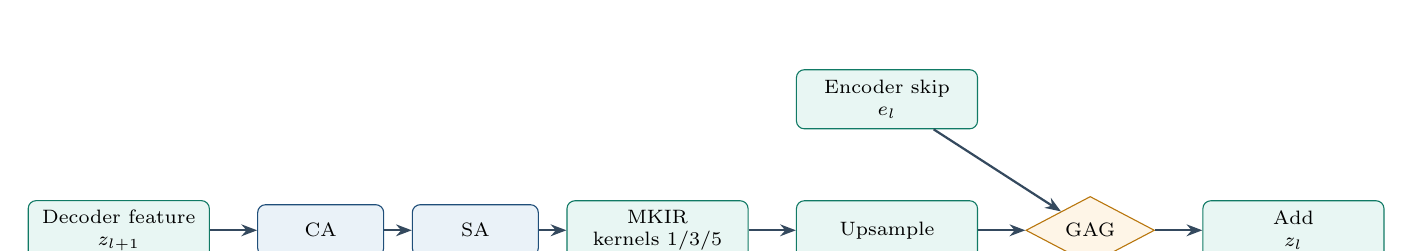
\begin{tikzpicture}[
  font=\scriptsize,
  block/.style={rectangle,rounded corners=1mm,draw=mainteal,fill=lightteal,minimum height=0.75cm,minimum width=2.3cm,align=center},
  small/.style={rectangle,rounded corners=1mm,draw=mainblue,fill=lightblue,minimum height=0.65cm,minimum width=1.6cm,align=center},
  gate/.style={diamond,aspect=1.9,draw=mainorange,fill=lightorange,minimum height=0.7cm,align=center},
  arr/.style={-{Stealth[length=2mm]},thick,draw=maingray}
]
\node[block] (x) {Decoder feature\\$z_{l+1}$};
\node[small,right=0.6cm of x] (ca) {CA};
\node[small,right=0.35cm of ca] (sa) {SA};
\node[block,right=0.35cm of sa] (mkir) {MKIR\\kernels 1/3/5};
\node[block,right=0.6cm of mkir] (up) {Upsample};
\node[block,above=0.9cm of up] (skip) {Encoder skip\\$e_l$};
\node[gate,right=0.6cm of up] (gag) {GAG};
\node[block,right=0.6cm of gag] (add) {Add\\$z_l$};

\draw[arr] (x) -- (ca);
\draw[arr] (ca) -- (sa);
\draw[arr] (sa) -- (mkir);
\draw[arr] (mkir) -- (up);
\draw[arr] (up) -- (gag);
\draw[arr] (skip) -- (gag);
\draw[arr] (gag) -- (add);
\end{tikzpicture}
}
\caption{Một decoder stage trong \modelname{} với GAG lọc skip feature trước khi hợp nhất.}
\label{fig:decoder-stage}
\end{figure}

\section{Deep supervision và hàm mất mát}

Segmentation branch có main mask và ba auxiliary masks ở các decoder stages trung gian. Các auxiliary heads dùng convolution $1\times1$ và được upsample về kích thước ảnh gốc để tính loss. Deep supervision giúp mô hình nhận tín hiệu phân đoạn ở nhiều mức phân giải, hữu ích khi dữ liệu nhỏ \citep{dsn,damknet}.

Tổng loss được viết như sau:
\[
\mathcal{L}=(1-\lambda)\mathcal{L}_{cls}+\lambda\mathcal{L}_{seg},
\]
trong đó
\[
\mathcal{L}_{seg}=\mathcal{L}_{BCE+Dice}(\hat{m})+w_a\sum_i \mathcal{L}_{BCE+Dice}(\hat{m}_i^{aux}).
\]
Theo thiết lập trong manuscript, $\lambda=0.8$ và $w_a=0.4$. Classification dùng focal loss để giảm ảnh hưởng của class imbalance; segmentation dùng tổng BCE và Dice loss để vừa học xác suất pixel vừa tối ưu overlap \citep{focalloss,diceloss,damknet}.

\section{Cơ chế xử lý ảnh normal}

\subsection{Class-balanced oversampling}

Trên BUSI, normal là lớp thiểu số với 133/780 ảnh. \modelname{} dùng deterministic class-balanced oversampling để tăng tần suất xuất hiện của từng lớp trong một epoch. Gọi $P_c$ là tỉ lệ mẫu của lớp $c$, replication factor được xác định bởi \citep{busi,aumente,damknet}
\[
RF_c=\left\lceil \frac{1}{P_c} \right\rceil.
\]
Oversampling không thay đổi nhãn và không tạo ca bệnh mới, nhưng giúp mô hình nhìn thấy các lớp cân bằng hơn. Khi kết hợp augmentation on-the-fly, các bản sao không hoàn toàn giống nhau ở mức input.

\subsection{Prediction-refining ở thời điểm suy luận}

Ngay cả khi mô hình đa nhiệm được huấn luyện tốt, hai head vẫn có thể mâu thuẫn. Prediction-refining xử lý mâu thuẫn này bằng hai quy tắc. Gọi $a$ là tỉ lệ pixel được segmentation head đánh dấu là lesion \citep{aumente,damknet}:
\[
a = \frac{1}{HW}\sum_{u=1}^{H}\sum_{v=1}^{W} \tilde{m}(u,v).
\]
Nếu $a<\tau$, vùng dương quá nhỏ được xem là không đủ bằng chứng cho lesion và nhãn được đặt về normal. Nếu nhãn cuối cùng là normal, mask được đặt rỗng.

\begin{algorithm}[H]
\caption{Prediction-refining cho đầu ra của \modelname{}}
\label{alg:refining}
\begin{algorithmic}[1]
\Require Class probabilities $p$, predicted mask probability $\hat{m}$, area threshold $\tau$
\State $\hat{y}\gets \arg\max_k p_k$
\State $\tilde{m}\gets \mathbb{I}\{\hat{m}>0.5\}$
\State $a\gets \frac{1}{HW}\sum_{u,v}\tilde{m}(u,v)$
\If{$a < \tau$}
  \State $\hat{y}\gets \text{normal}$
\EndIf
\If{$\hat{y}=\text{normal}$}
  \State $\tilde{m}\gets \mathbf{0}_{H\times W}$
\EndIf
\State \Return refined label $\hat{y}$ and refined mask $\tilde{m}$
\end{algorithmic}
\end{algorithm}

\begin{figure}[H]
\centering
\resizebox{\textwidth}{!}{%
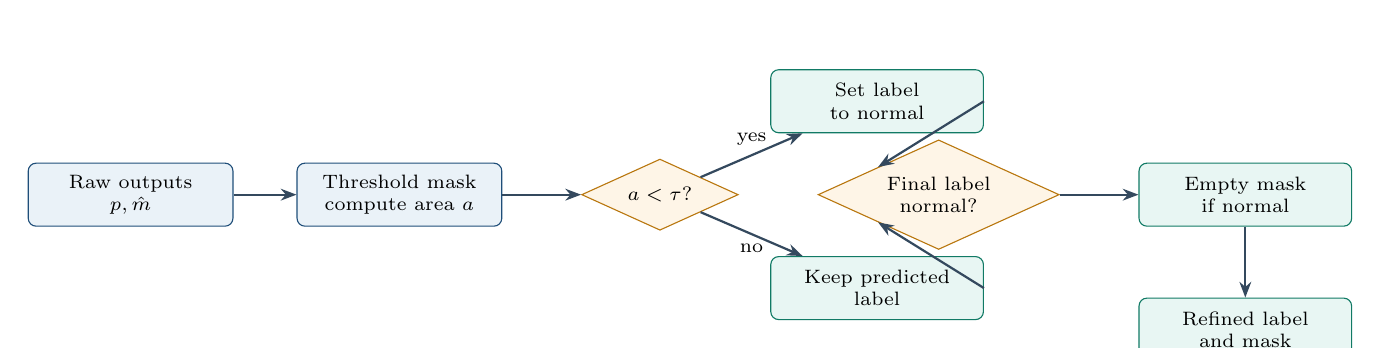
\begin{tikzpicture}[
  font=\scriptsize,
  block/.style={rectangle,rounded corners=1mm,draw=mainblue,fill=lightblue,minimum height=0.8cm,minimum width=2.6cm,align=center},
  decision/.style={diamond,aspect=2.2,draw=mainorange,fill=lightorange,minimum height=0.9cm,align=center},
  outnode/.style={rectangle,rounded corners=1mm,draw=mainteal,fill=lightteal,minimum height=0.8cm,minimum width=2.7cm,align=center},
  arr/.style={-{Stealth[length=2mm]},thick,draw=maingray}
]
\node[block] (pred) {Raw outputs\\$p,\hat{m}$};
\node[block,right=0.8cm of pred] (bin) {Threshold mask\\compute area $a$};
\node[decision,right=1.0cm of bin] (d1) {$a<\tau$?};
\node[outnode,above right=0.55cm and 0.9cm of d1] (normal) {Set label\\to normal};
\node[outnode,below right=0.55cm and 0.9cm of d1] (keep) {Keep predicted\\label};
\node[decision,right=1.0cm of d1] (d2) {Final label\\normal?};
\node[outnode,right=1.0cm of d2] (zero) {Empty mask\\if normal};
\node[outnode,below=0.9cm of zero] (final) {Refined label\\and mask};

\draw[arr] (pred) -- (bin);
\draw[arr] (bin) -- (d1);
\draw[arr] (d1) -- node[above]{yes} (normal);
\draw[arr] (d1) -- node[below]{no} (keep);
\draw[arr] (normal.east) -- (d2.north west);
\draw[arr] (keep.east) -- (d2.south west);
\draw[arr] (d2) -- (zero);
\draw[arr] (zero) -- (final);
\end{tikzpicture}
}
\caption{Logic prediction-refining để đồng bộ nhãn normal và mask dự đoán.}
\label{fig:refining-flow}
\end{figure}

% =========================================================
\chapter{Thiết lập thực nghiệm}

\section{Dữ liệu}

Thực nghiệm sử dụng Breast Ultrasound Images Dataset (BUSI), gồm 780 ảnh thuộc ba lớp: 437 benign, 210 malignant và 133 normal. Ảnh benign và malignant có mask tổn thương do chuyên gia gán nhãn; ảnh normal được gán mask rỗng. Điểm quan trọng trong protocol của \modelname{} là ảnh normal được giữ trong train, validation và test cho cả hai tác vụ, thay vì bị loại khỏi segmentation như các thiết lập tumor-only \citep{busi,damknet}.

Tất cả ảnh được resize về 224$\times$224. Việc cố định input size giúp so sánh FLOPs và latency công bằng hơn giữa các cấu hình width. Tuy nhiên, resize cũng là một nguồn sai lệch tiềm năng đối với lesion nhỏ; do đó các kết quả cần được hiểu trong phạm vi input resolution này \citep{damknet}.

\section{Baseline}

Báo cáo sử dụng ba nhóm baseline:

\begin{enumerate}
  \item \textbf{MedNet}: classifier đơn nhiệm, dự đoán benign/malignant/normal nhưng không tạo mask \citep{mednet}.
  \item \textbf{MK-UNet}: segmenter đơn nhiệm, đánh giá trên ảnh benign/malignant và không xử lý normal scans \citep{mkunet}.
  \item \textbf{RCBAMMNet}: ablation dùng cùng shared encoder nhưng thay multi-kernel decoder bằng inception-style depthwise-separable decoder và CBAM-gated skips, nhằm cô lập tác động của decoder choice \citep{cbam,damknet}.
\end{enumerate}

Ngoài ra, MedNet + MK-UNet được xem như pipeline hai mô hình tự nhiên nếu muốn có cả classification và segmentation bằng các mô hình đơn nhiệm \citep{mednet,mkunet,damknet}.

\section{Chi tiết huấn luyện}

Theo manuscript, các mô hình được huấn luyện trong 100 epochs với AdamW, weight decay $10^{-4}$, cosine annealing với learning rate tối thiểu $10^{-6}$ và batch size 16. Với \modelname{} và RCBAMMNet, learning rate là $3\times10^{-4}$, $\lambda=0.8$, deep supervision weight $w_a=0.4$, oversampling trong huấn luyện và prediction-refining ở suy luận. MedNet dùng cùng công thức classification. MK-UNet dùng recipe riêng của nó với learning rate $10^{-4}$, multi-scale training và structure loss trong cùng ngân sách epoch \citep{mednet,mkunet,damknet}.

Best checkpoint được chọn theo validation loss cho multi-task models, theo Dice cho MK-UNet và theo accuracy cho MedNet. Điểm đáng chú ý là efficiency được đo bằng cùng profiler ở input 224$\times$224 để các cột tham số và GMac có thể so sánh trực tiếp \citep{damknet}.

\section{Metric đánh giá}

Phân loại được đánh giá bằng accuracy, one-vs-rest ROC-AUC và F1 theo lớp. Phân đoạn được đánh giá bằng Dice và IoU. Báo cáo dùng lesion Dice trung bình trên benign/malignant để so sánh với segmenters vốn loại normal, đồng thời dùng normal Dice để đo khả năng giữ mask rỗng trên ảnh normal \citep{diceloss,taha2015,damknet}.

\begin{cautionbox}{Cách đọc metric trong CAD y khoa}
Accuracy không đủ để đánh giá hệ thống CAD. Một mô hình có accuracy cao vẫn có thể không phù hợp nếu bỏ sót nhiều ca malignant hoặc tạo mask giả trên normal. Vì vậy, kết quả phải được đọc cùng lesion Dice, normal Dice, F1 theo lớp, specificity và false-positive rate trên normal scans.
\end{cautionbox}

% =========================================================
\chapter{Kết quả thực nghiệm}

\section{So sánh chính: một mô hình cho toàn bộ pipeline}

Bảng~\ref{tab:main-comparison} trình bày so sánh chính trên BUSI. \modelnames{} đạt accuracy 85.83\%, AUC 0.965 và lesion Dice 79.37\% với 2.25M tham số và 1.50 GMac. So với pipeline MedNet + MK-UNet, \modelnames{} dùng ít tham số và compute hơn, nhưng vẫn cung cấp cả phân loại, phân đoạn và xử lý normal trong một lần suy luận \citep{mednet,mkunet,damknet}.

\begin{table}[H]
\centering
\caption{So sánh chính trên BUSI. FLOPs được báo cáo dưới dạng GMac tại input 224$\times$224. Dấu \checkmark{} ở cột Normal nghĩa là mô hình giữ và xử lý normal scans trong pipeline.}
\label{tab:main-comparison}
\resizebox{\textwidth}{!}{%
\begin{tabular}{lccccccc}
\toprule
\textbf{Phương pháp} & \textbf{Params (M)} & \textbf{GMac} & \textbf{Tác vụ} & \textbf{Acc.} & \textbf{AUC} & \textbf{Dice$_{les}$} & \textbf{Normal} \\
\midrule
MedNet & 3.27 & 2.02 & Cls & 81.67 & 0.936 & -- & $\times$ \\
MK-UNet & 0.32 & 0.25 & Seg & -- & -- & 78.04 & $\times$ \\
MedNet + MK-UNet & 3.59 & 2.27 & Cls+Seg & 81.67 & 0.936 & 78.04 & $\times$ \\
\modelname{}-T & 0.63 & 0.46 & All & 78.33 & 0.942 & 77.46 & \checkmark \\
\modelname{}-S & 2.25 & 1.50 & All & \textbf{85.83} & \textbf{0.965} & \textbf{79.37} & \checkmark \\
\modelname{} & 8.51 & 5.36 & All & 88.33 & 0.975 & 81.97 & \checkmark \\
\bottomrule
\end{tabular}}
\end{table}

Kết quả này nên được đọc theo đúng phạm vi. MK-UNet vẫn là segmenter nhẹ hơn nếu chỉ cần segmentation. Đóng góp của \modelname{} không phải là đánh bại mọi segmenter trên chi phí segmentation-only, mà là cung cấp một pipeline đầy đủ trong một mô hình nhỏ hơn hai-model pipeline \citep{mkunet,damknet}.

\section{Ablation: oversampling và prediction-refining}

Bảng~\ref{tab:os-pr-ablation} cho thấy normal scans cần một cơ chế rõ ràng. Multi-task training đơn thuần ở full width đạt Dice normal 42.86\%, tức segmentation head vẫn vẽ vùng dương trên ảnh khỏe mạnh. Oversampling cải thiện accuracy và lesion Dice, nhưng không tự nó giải quyết normal segmentation. Prediction-refining mới là thành phần quyết định nâng Dice normal lên 85.71\% khi dùng riêng, và lên 90.48\% khi kết hợp với oversampling \citep{aumente,damknet}.

\begin{table}[H]
\centering
\caption{Ảnh hưởng của oversampling (OS) và prediction-refining (PR) tại width $w=1.0$.}
\label{tab:os-pr-ablation}
\begin{tabular}{lccc}
\toprule
\textbf{Cấu hình} & \textbf{Acc.} & \textbf{Dice$_{les}$} & \textbf{Dice$_{norm}$} \\
\midrule
Multi-task & 81.67 & 79.16 & 42.86 \\
+ OS & 87.50 & 81.97 & 33.33 \\
+ PR & 81.67 & 78.41 & 85.71 \\
+ OS + PR & \textbf{88.33} & \textbf{81.97} & \textbf{90.48} \\
\bottomrule
\end{tabular}
\end{table}

Bảng này là bằng chứng quan trọng cho luận điểm của báo cáo: multi-task learning không tự động tạo ra normal-aware behavior. Hai output heads được tối ưu để đúng riêng lẻ, không tự động bị ràng buộc phải đồng ý. Prediction-refining đưa ràng buộc miền ứng dụng vào hệ thống: nếu ảnh được xem là normal thì mask phải rỗng \citep{aumente,damknet}.

\section{Ablation: lựa chọn decoder}

\begin{table}[H]
\centering
\caption{So sánh decoder trên cùng shared encoder.}
\label{tab:decoder-ablation}
\resizebox{\textwidth}{!}{%
\begin{tabular}{lccccc}
\toprule
\textbf{Decoder} & \textbf{Params (M)} & \textbf{GMac} & \textbf{Acc.} & \textbf{AUC} & \textbf{Dice$_{les}$} \\
\midrule
Inception / CBAM-RI (RCBAMMNet) & 6.56 & 10.21 & 85.83 & 0.957 & 74.76 \\
Multi-kernel (\modelname{}-S) & \textbf{2.25} & \textbf{1.50} & 85.83 & \textbf{0.965} & \textbf{79.37} \\
\bottomrule
\end{tabular}}
\end{table}

Multi-kernel decoder đạt cùng accuracy nhưng AUC và lesion Dice cao hơn, đồng thời dùng khoảng một phần ba tham số và khoảng một phần bảy compute so với inception-style decoder. Kết quả này phù hợp với giả thuyết kiến trúc: lesion siêu âm biến thiên kích thước mạnh, nên nhiều kernel song song giúp decoder đọc cả chi tiết nhỏ và ngữ cảnh rộng với chi phí thấp \citep{mkunet,damknet}.

\section{Đường đánh đổi theo width multiplier}

Width multiplier tạo một họ mô hình từ 0.63M đến 8.51M tham số. Bước từ \modelname{}-T lên \modelname{}-S tạo cải thiện lớn: accuracy tăng từ 78.33\% lên 85.83\%, lesion Dice tăng từ 77.46\% lên 79.37\%. Bước từ \modelname{}-S lên full model tăng accuracy từ 85.83\% lên 88.33\% và Dice từ 79.37\% lên 81.97\%, nhưng đổi lại tham số tăng gần bốn lần và compute tăng hơn ba lần. Vì vậy, \modelname{}-S là điểm gối hợp lý trên đường đánh đổi accuracy--cost \citep{damknet}.

\section{Kết quả theo lớp}

\begin{table}[H]
\centering
\caption{Kết quả theo lớp của mô hình đề xuất sau oversampling và prediction-refining.}
\label{tab:per-class}
\begin{tabular}{lcc}
\toprule
\textbf{Model} & \textbf{Dice (benign/malignant/normal)} & \textbf{F1 (benign/malignant/normal)} \\
\midrule
\modelname{}-S & 79.2 / 79.6 / 81.0 & 0.878 / 0.806 / 0.872 \\
\modelname{} & 82.3 / 81.3 / 90.5 & 0.903 / 0.786 / 0.950 \\
\bottomrule
\end{tabular}
\end{table}

Malignant là lớp khó hơn trong phân loại, với F1 0.806 ở \modelname{}-S và 0.786 ở full model. Điều này có ý nghĩa lâm sàng: cải thiện accuracy tổng thể không nên là mục tiêu duy nhất; cần ưu tiên giảm false-negative malignant vì bỏ sót ác tính có hậu quả nghiêm trọng hơn báo động giả \citep{globocan,damknet}.

\section{False positive trên normal scans và độ nhạy threshold}

Theo manuscript, prediction-refining giảm false-positive rate trên normal scans từ 23.8\% xuống 14.3\% cho \modelname{}-S, và từ 14.3\% xuống 9.5\% cho full model. Specificity tương ứng tăng lên 0.86 và 0.90. Ngoài ra, các metric sau refinement ổn định khi $\tau\in[5\times10^{-4},5\times10^{-3}]$, và chỉ suy giảm rõ khi $\tau\geq10^{-2}$ do các lesion thật nhỏ bắt đầu bị relabel thành normal \citep{damknet}.

\section{Runtime}

Ở batch size 1 trên CPU, latency được báo cáo lần lượt là 37 ms, 70 ms và 138 ms cho \modelname{}-T, \modelname{}-S và full \modelname{}. Điều này củng cố mục tiêu deployment: mô hình nhỏ nhất nằm trong vùng tương tác thời gian thực, trong khi \modelname{}-S vẫn đủ nhanh cho một CAD pipeline nhẹ \citep{damknet}.

\section{Bằng chứng định tính}

Các hình định tính nên được đặt trong thư mục \code{figures/}. Báo cáo cuối nên gồm ít nhất ba nhóm hình: prediction examples, Grad-CAM và threshold/runtime plot. Nếu chưa có hình, các khung dưới đây sẽ hiển thị placeholder để tránh lỗi biên dịch.

\begin{figure}[H]
\centering
\figplaceholder[width=0.92\textwidth]{damk_predictions_three_classes.png}
\caption{Ví dụ dự đoán của \modelname{} trên ba lớp benign, malignant và normal. Mỗi hàng nên gồm input, ground-truth mask và predicted mask sau prediction-refining.}
\label{fig:qualitative-predictions}
\end{figure}

\begin{figure}[H]
\centering
\figplaceholder[width=0.92\textwidth]{damk_gradcam_three_classes.png}
\caption{Grad-CAM từ encoder stage cuối cho ba trường hợp đại diện. Với benign/malignant, activation nên tập trung quanh lesion; với normal, activation lý tưởng là phân tán và không tạo vùng dương rõ.}
\label{fig:gradcam}
\end{figure}

\begin{figure}[H]
\centering
\figplaceholder[width=0.75\textwidth]{threshold_sensitivity.png}
\caption{Độ nhạy của prediction-refining theo ngưỡng diện tích $\tau$. Hình nên thể hiện accuracy, normal Dice và normal false-positive rate theo thang log của $\tau$.}
\label{fig:threshold-sensitivity}
\end{figure}

% =========================================================
\chapter{Bàn luận}

\section{Vai trò của shared encoder}

Kết quả cho thấy shared encoder là thành phần làm cho một mô hình duy nhất có thể thay thế pipeline hai mô hình ở mức chi phí thấp hơn. Classification và segmentation đều cần feature extractor mạnh; nếu dùng hai mô hình riêng, chi phí feature extraction bị lặp. \modelname{} loại bỏ phần lặp này bằng một encoder chung, sau đó thêm classification head và decoder tương đối nhẹ \citep{zhou,aumente,damknet}.

Tuy nhiên, shared encoder không chỉ có ý nghĩa tiết kiệm compute. Khi encoder nhận gradient từ cả nhãn toàn ảnh và mask pixel-level, biểu diễn học được có xu hướng kết hợp thông tin ngữ nghĩa và không gian. Điều này phù hợp với bản chất của ảnh siêu âm vú: lesion vừa là đối tượng cần định vị, vừa là bằng chứng cho nhãn \citep{busi,aumente,damknet}.

\section{Vì sao normal-aware design là bắt buộc}

Ablation cho thấy nếu chỉ dùng multi-task training, normal Dice vẫn thấp. Lý do là loss không cấm hai đầu ra mâu thuẫn nhau. Classification loss chỉ quan tâm nhãn, segmentation loss chỉ quan tâm overlap pixel. Nếu ảnh normal tạo một vùng mask dương nhỏ, loss tổng có thể vẫn không phạt đủ mạnh để loại bỏ hành vi này, đặc biệt khi normal là lớp thiểu số \citep{aumente,damknet}.

Prediction-refining đưa tri thức miền ứng dụng vào suy luận: ảnh normal phải có mask rỗng. Đây là một ràng buộc đơn giản nhưng có ý nghĩa lớn. Điểm cần thận trọng là threshold $\tau$ phải được chọn trên validation set và kiểm tra độ nhạy. Nếu $\tau$ quá cao, hệ thống có thể xóa lesion nhỏ thật; nếu quá thấp, false-positive mask trên normal vẫn tồn tại \citep{aumente,damknet}.

\section{Ý nghĩa của multi-kernel decoder}

Multi-kernel decoder tốt hơn inception-style decoder trên cùng encoder cả về Dice lesion lẫn compute. Điều này cho thấy hiệu quả không chỉ đến từ shared encoder, mà còn từ cách khôi phục mask. Các kernel $1\times1$, $3\times3$ và $5\times5$ trong MKIR cho phép mô hình kết hợp nhiều receptive fields mà không cần tăng mạnh số kênh. Đối với ảnh siêu âm vú, đây là lựa chọn hợp lý vì lesion có thể thay đổi từ vùng nhỏ, rõ biên đến vùng rộng, mờ biên \citep{mkunet,damknet}.

\section{Diễn giải lâm sàng của lỗi}

Các lỗi trong CAD y khoa không đối xứng. Nhầm malignant thành benign hoặc normal có thể gây chậm trễ chẩn đoán. Nhầm benign thành malignant có thể gây báo động giả và tăng can thiệp không cần thiết. Vẽ mask giả trên normal làm giảm độ tin cậy và có thể tạo follow-up không cần thiết. Vì vậy, tối ưu accuracy tổng thể là chưa đủ. Các vòng cải tiến tiếp theo nên ưu tiên malignant sensitivity, normal false-positive rate và calibration xác suất \citep{globocan,aumente,damknet}.

\section{Không nên diễn giải quá mức kết quả}

Kết quả trên BUSI là bằng chứng quan trọng nhưng chưa đủ cho kết luận triển khai. BUSI là public dataset quy mô nhỏ, và các ảnh có thể không đại diện cho mọi thiết bị, bệnh viện hoặc quần thể bệnh nhân. Ngoài ra, paper chưa cung cấp external validation độc lập. Do đó, kết luận đúng là \modelname{} tạo ra một baseline compact và clinically more complete hơn segmentation-only hoặc classification-only, không phải một hệ thống đã sẵn sàng dùng trong lâm sàng \citep{busi,damknet}.

% =========================================================
\chapter{Giới hạn và đe dọa đến tính hợp lệ}

\section{Giới hạn dữ liệu}

Đánh giá hiện dựa trên một dataset công khai. Public datasets thường có quy mô nhỏ, protocol thu ảnh không đồng nhất và có thể không phản ánh đầy đủ phân bố lâm sàng thực tế. Việc thiếu external validation làm giới hạn khả năng kết luận về generalization \citep{busi,damknet}.

\section{Giới hạn protocol}

Một số baseline được so sánh bằng published results hoặc recipe riêng, không hoàn toàn là same-protocol re-run. Điều này là hợp lý để định vị phương pháp, nhưng chưa đủ để khẳng định ưu thế tuyệt đối. Một nghiên cứu tiếp theo nên tái chạy các multi-task baselines trong cùng split, cùng input size, cùng metric và cùng profiler \citep{mkunet,mednet,damknet}.

\section{Giới hạn của prediction-refining}

Prediction-refining dùng threshold diện tích cố định. Dù paper báo cáo metric ổn định trên một khoảng threshold rộng, cơ chế này vẫn có rủi ro với lesion rất nhỏ. Một hướng tốt hơn là học adaptive threshold hoặc thêm consistency loss trong huấn luyện để giảm phụ thuộc vào hậu xử lý \citep{aumente,damknet}.

\section{Giới hạn thống kê}

Báo cáo hiện chưa nhấn mạnh đủ mean/std qua nhiều random seeds hoặc cross-validation. Với dataset nhỏ, kết quả có thể nhạy với split và seed. Do đó, trước khi đưa ra kết luận mạnh, cần báo cáo độ lệch chuẩn, confidence interval và kiểm định thống kê cho các ablation chính.

% =========================================================
\chapter{Kết luận và hướng phát triển}

\section{Kết luận}

Báo cáo đã phân tích \modelname{} như một mô hình CAD nhẹ, đa nhiệm và normal-aware cho ảnh siêu âm vú. Điểm mạnh của hướng tiếp cận này là dùng một shared encoder cho cả phân loại và phân đoạn, dùng multi-kernel decoder để khôi phục mask với chi phí thấp, và dùng oversampling cùng prediction-refining để xử lý normal scans. Trên BUSI, \modelname{}-S đạt 85.83\% accuracy, AUC 0.965 và 79.37\% lesion Dice với 2.25M tham số và 1.50 GMac. Full \modelname{} đạt 88.33\% accuracy và 81.97\% lesion Dice, nhưng với chi phí cao hơn đáng kể \citep{busi,damknet}.

Kết luận quan trọng nhất là multi-task learning không tự động giải quyết bài toán normal. Normal-aware behavior cần cơ chế riêng, và prediction-refining là thành phần có tác động quyết định lên normal Dice. Vì vậy, khi đánh giá CAD siêu âm vú, cần đọc đồng thời classification metrics, lesion segmentation metrics và normal-specific metrics \citep{aumente,damknet}.

\section{Hướng phát triển}

Các hướng phát triển nên được ưu tiên theo thứ tự sau:

\begin{enumerate}
  \item \textbf{Đánh giá thống kê chắc hơn}: chạy nhiều seeds hoặc cross-validation, báo cáo mean/std và confidence interval.
  \item \textbf{External validation}: kiểm định trên dataset khác như BUS-BRA hoặc dữ liệu nội bộ đa thiết bị.
  \item \textbf{Adaptive refinement}: thay threshold cố định bằng ngưỡng học được hoặc uncertainty-aware criterion.
  \item \textbf{Consistency loss}: thêm ràng buộc huấn luyện giữa class prediction và mask area để giảm mâu thuẫn đầu ra trước hậu xử lý.
  \item \textbf{Tối ưu clinical operating point}: ưu tiên malignant sensitivity và giảm false positives trên normal thông qua threshold theo mục tiêu lâm sàng.
  \item \textbf{Đánh giá triển khai}: đo latency, memory footprint, calibration và robustness trên CPU, GPU thấp, edge device hoặc point-of-care hardware.
\end{enumerate}

% =========================================================
\appendix
\chapter{Gợi ý tổ chức thư mục nộp}

\begin{verbatim}
project/
  main.tex
  final_report.pdf
  figures/
    damk_predictions_three_classes.png
    damk_gradcam_three_classes.png
    threshold_sensitivity.png
    confusion_matrix_raw.png
    confusion_matrix_refined.png
\end{verbatim}

\chapter{Checklist trước khi nộp}

\begin{itemize}
  \item Kiểm tra tất cả số liệu trong bảng khớp với kết quả thực nghiệm hoặc paper gốc.
  \item Không trộn tên MK-MNet và DAMK-Net nếu không giải thích rõ.
  \item Không tuyên bố ``clinical-ready'' nếu chưa có external validation.
  \item Bảo đảm mọi hình có caption mô tả input, ground truth, prediction và ý nghĩa.
  \item Bảo đảm mọi citation trong phần related work có mục tương ứng trong tài liệu tham khảo.
  \item Biên dịch bằng XeLaTeX hoặc LuaLaTeX.
\end{itemize}

% =========================================================
\clearpage
\begin{thebibliography}{99}
\addcontentsline{toc}{chapter}{Tài liệu tham khảo}

\bibitem[Al-Dhabyani et~al.(2020)]{busi}
Al-Dhabyani, W., Gomaa, M., Khaled, H. and Fahmy, A. (2020)
`Dataset of breast ultrasound images',
\textit{Data in Brief}, 28, article 104863.
\href{https://doi.org/10.1016/j.dib.2019.104863}{doi:10.1016/j.dib.2019.104863}.

\bibitem[Aumente-Maestro et~al.(2025)]{aumente}
Aumente-Maestro, C., Díez, J. and Remeseiro, B. (2025)
`A multi-task framework for breast cancer segmentation and classification in ultrasound imaging',
\textit{Computer Methods and Programs in Biomedicine}, 260, article 108540.
\href{https://doi.org/10.1016/j.cmpb.2024.108540}{doi:10.1016/j.cmpb.2024.108540}.

\bibitem[Chollet(2017)]{xception}
Chollet, F. (2017)
`Xception: Deep learning with depthwise separable convolutions',
in \textit{Proceedings of the IEEE Conference on Computer Vision and Pattern Recognition}, pp. 1251--1258.
\href{https://doi.org/10.1109/CVPR.2017.195}{doi:10.1109/CVPR.2017.195}.

\bibitem[Ferdous et~al.(2025)]{mednet}
Ferdous, M., Mahmud, S. and Shimul, M.E.Z. (2025)
`MedNet: a lightweight attention-augmented CNN for medical image classification',
\textit{Scientific Reports}, 15, article 41936.
\href{https://doi.org/10.1038/s41598-025-25857-w}{doi:10.1038/s41598-025-25857-w}.

\bibitem[Howard et~al.(2017)]{mobilenet}
Howard, A.G., Zhu, M., Chen, B., Kalenichenko, D., Wang, W., Weyand, T., Andreetto, M. and Adam, H. (2017)
`MobileNets: Efficient convolutional neural networks for mobile vision applications',
\textit{arXiv preprint}.
\href{https://doi.org/10.48550/arXiv.1704.04861}{doi:10.48550/arXiv.1704.04861}.

\bibitem[Lee et~al.(2015)]{dsn}
Lee, C.-Y., Xie, S., Gallagher, P., Zhang, Z. and Tu, Z. (2015)
`Deeply-supervised nets',
in \textit{Proceedings of the 18th International Conference on Artificial Intelligence and Statistics}, PMLR 38, pp. 562--570.
Available at: \url{https://proceedings.mlr.press/v38/lee15a.html}.

\bibitem[Le(2026)]{damknet}
Le, Q. (2026)
`DAMK-Net: A compact multi-task network for breast ultrasound classification and segmentation',
\textit{Springer Lecture Notes in Computer Science manuscript}. Unpublished manuscript provided in the project repository; no public DOI available at the time of report preparation.

\bibitem[Lin et~al.(2017)]{focalloss}
Lin, T.-Y., Goyal, P., Girshick, R., He, K. and Dollár, P. (2017)
`Focal loss for dense object detection',
in \textit{Proceedings of the IEEE International Conference on Computer Vision}, pp. 2980--2988.
\href{https://doi.org/10.1109/ICCV.2017.324}{doi:10.1109/ICCV.2017.324}.

\bibitem[Milletari et~al.(2016)]{diceloss}
Milletari, F., Navab, N. and Ahmadi, S.-A. (2016)
`V-Net: Fully convolutional neural networks for volumetric medical image segmentation',
in \textit{2016 Fourth International Conference on 3D Vision}, pp. 565--571.
\href{https://doi.org/10.1109/3DV.2016.79}{doi:10.1109/3DV.2016.79}.

\bibitem[Müller and Hutter(2021)]{trivialaugment}
Müller, S.G. and Hutter, F. (2021)
`TrivialAugment: Tuning-free yet state-of-the-art data augmentation',
\textit{arXiv preprint}.
\href{https://doi.org/10.48550/arXiv.2103.10158}{doi:10.48550/arXiv.2103.10158}.

\bibitem[Oktay et~al.(2018)]{attnunet}
Oktay, O., Schlemper, J., Folgoc, L.L., Lee, M., Heinrich, M., Misawa, K., Mori, K., McDonagh, S., Hammerla, N.Y., Kainz, B., Glocker, B. and Rueckert, D. (2018)
`Attention U-Net: Learning where to look for the pancreas',
\textit{arXiv preprint}.
\href{https://doi.org/10.48550/arXiv.1804.03999}{doi:10.48550/arXiv.1804.03999}.

\bibitem[Rahman and Marculescu(2025)]{mkunet}
Rahman, M.M. and Marculescu, R. (2025)
`MK-UNet: Multi-kernel lightweight CNN for medical image segmentation',
in \textit{2025 IEEE/CVF International Conference on Computer Vision Workshops}, pp. 1053--1062.
\href{https://doi.org/10.1109/ICCVW69036.2025.00114}{doi:10.1109/ICCVW69036.2025.00114}.

\bibitem[Ronneberger et~al.(2015)]{unet}
Ronneberger, O., Fischer, P. and Brox, T. (2015)
`U-Net: Convolutional networks for biomedical image segmentation',
in \textit{Medical Image Computing and Computer-Assisted Intervention -- MICCAI 2015}, LNCS 9351, pp. 234--241.
\href{https://doi.org/10.1007/978-3-319-24574-4_28}{doi:10.1007/978-3-319-24574-4\_28}.

\bibitem[Sandler et~al.(2018)]{mobilenetv2}
Sandler, M., Howard, A., Zhu, M., Zhmoginov, A. and Chen, L.-C. (2018)
`MobileNetV2: Inverted residuals and linear bottlenecks',
in \textit{Proceedings of the IEEE Conference on Computer Vision and Pattern Recognition}, pp. 4510--4520.
\href{https://doi.org/10.1109/CVPR.2018.00474}{doi:10.1109/CVPR.2018.00474}.

\bibitem[Selvaraju et~al.(2017)]{gradcam}
Selvaraju, R.R., Cogswell, M., Das, A., Vedantam, R., Parikh, D. and Batra, D. (2017)
`Grad-CAM: Visual explanations from deep networks via gradient-based localization',
in \textit{Proceedings of the IEEE International Conference on Computer Vision}, pp. 618--626.
\href{https://doi.org/10.1109/ICCV.2017.74}{doi:10.1109/ICCV.2017.74}.

\bibitem[Sung et~al.(2021)]{globocan}
Sung, H., Ferlay, J., Siegel, R.L., Laversanne, M., Soerjomataram, I., Jemal, A. and Bray, F. (2021)
`Global cancer statistics 2020: GLOBOCAN estimates of incidence and mortality worldwide for 36 cancers in 185 countries',
\textit{CA: A Cancer Journal for Clinicians}, 71(3), pp. 209--249.
\href{https://doi.org/10.3322/caac.21660}{doi:10.3322/caac.21660}.

\bibitem[Taha and Hanbury(2015)]{taha2015}
Taha, A.A. and Hanbury, A. (2015)
`Metrics for evaluating 3D medical image segmentation: analysis, selection, and tool',
\textit{BMC Medical Imaging}, 15, article 29.
\href{https://doi.org/10.1186/s12880-015-0068-x}{doi:10.1186/s12880-015-0068-x}.

\bibitem[Tupper and Gagné(2024)]{augmentation}
Tupper, A. and Gagné, C. (2024)
`Analyzing data augmentation for medical images: A case study in ultrasound images',
\textit{arXiv preprint}.
\href{https://doi.org/10.48550/arXiv.2403.09828}{doi:10.48550/arXiv.2403.09828}.

\bibitem[Woo et~al.(2018)]{cbam}
Woo, S., Park, J., Lee, J.-Y. and Kweon, I.S. (2018)
`CBAM: Convolutional block attention module',
in \textit{Computer Vision -- ECCV 2018}, LNCS 11211, pp. 3--19.
\href{https://doi.org/10.1007/978-3-030-01234-2_1}{doi:10.1007/978-3-030-01234-2\_1}.

\bibitem[Zhang et~al.(2018)]{shufflenet}
Zhang, X., Zhou, X., Lin, M. and Sun, J. (2018)
`ShuffleNet: An extremely efficient convolutional neural network for mobile devices',
in \textit{Proceedings of the IEEE Conference on Computer Vision and Pattern Recognition}, pp. 6848--6856.
\href{https://doi.org/10.1109/CVPR.2018.00716}{doi:10.1109/CVPR.2018.00716}.

\bibitem[Zhou et~al.(2018)]{unetpp}
Zhou, Z., Rahman Siddiquee, M.M., Tajbakhsh, N. and Liang, J. (2018)
`UNet++: A nested U-Net architecture for medical image segmentation',
in \textit{Deep Learning in Medical Image Analysis and Multimodal Learning for Clinical Decision Support}, LNCS 11045, pp. 3--11.
\href{https://doi.org/10.1007/978-3-030-00889-5_1}{doi:10.1007/978-3-030-00889-5\_1}.

\bibitem[Zhou et~al.(2021)]{zhou}
Zhou, Y., Chen, H., Li, Y., Liu, Q., Xu, X., Wang, S., Yap, P.-T. and Shen, D. (2021)
`Multi-task learning for segmentation and classification of tumors in 3D automated breast ultrasound images',
\textit{Medical Image Analysis}, 70, article 101918.
\href{https://doi.org/10.1016/j.media.2020.101918}{doi:10.1016/j.media.2020.101918}.

\end{thebibliography}

\end{document}
